\documentclass{article}
\usepackage{listings}
\usepackage{graphicx}
\title{FWC RTL ASSIGNMENT-1}
\author{A.CHINNAPA REDDY}
\date{\today}
\begin{document}
\maketitle
\section{Module Code}
\begin{lstlisting}
`timescale 1ns / 1ps

module downcounter(
  
// Inputs
input   wire    [7:0]   in,
input   wire            clk,
input   wire            latch,
input   wire            dec,
input   wire            div,
// Outputs
output  wire            zero,
// Internal
output  reg     [7:0]   count
);



always @(posedge clk)
begin
    if(latch)
        count <= in;
    else if(dec)
        count <= (count==8'd0)?8'd0:count - 1;
    else if(div)
        count <= count >> 1;
end


assign zero = (count == 0);
endmodule
\end{lstlisting}




\section{Testbench Code}
\begin{lstlisting}
`timescale 1ns / 1ps

`include "downcounter.v"

module downcounter$_$tb;
reg     [7:0]   in;
reg             clk, latch, dec, div; 
wire    [7:0]   count;
wire            zero;

downcounter UUT(
    .in(in),
    .clk(clk),
    .latch(latch),
    .dec(dec),
    .div(div),
    .count(count),
    .zero(zero)
);

initial begin
    clk = 1'b0;
    forever #1 clk = ~clk; 
end


initial begin
    in= 8'd16; latch = 1'b1; dec = 1'b0; div = 1'b0;
    #2 in=8'd0;latch = 1'b0;
    #4.5  div = 1'b1;
    #6.5   div=1'b0;
    #5 $finish;
end
endmodule
\end{lstlisting}
\section{Timing Circuit}
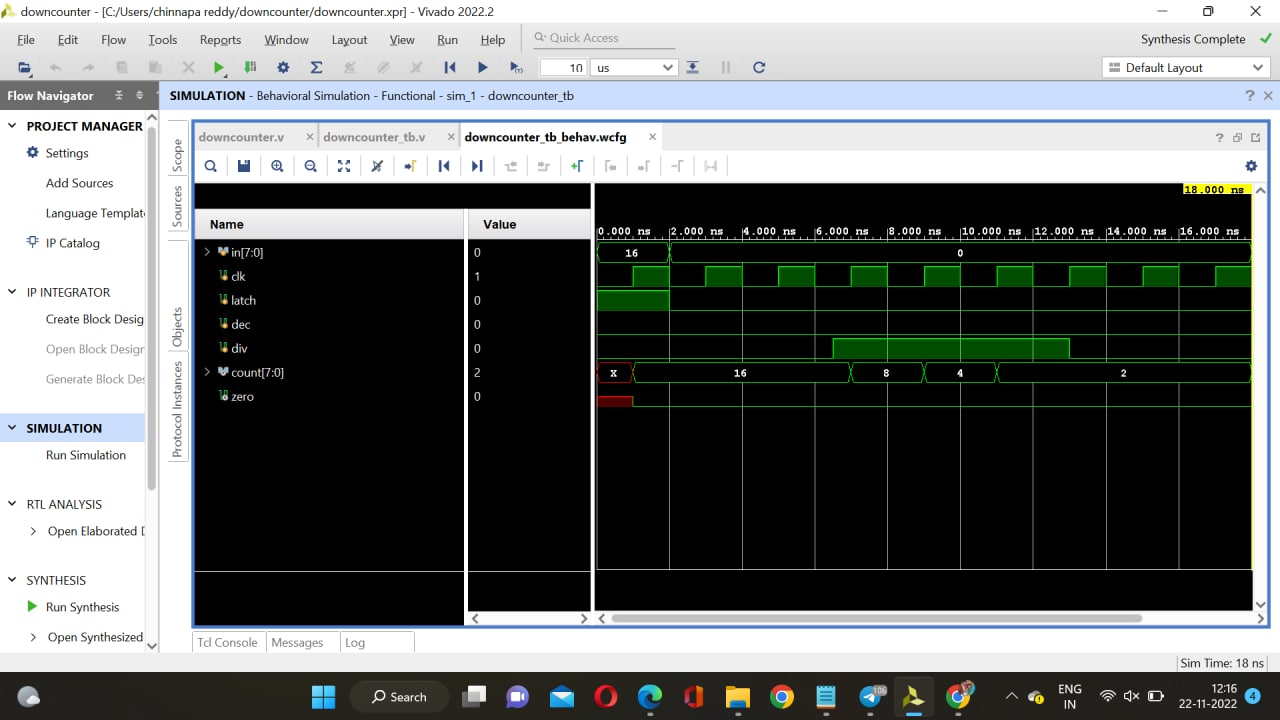
\includegraphics[width=1\columnwidth]{figs/1.jpg}
\section{Device diagram}
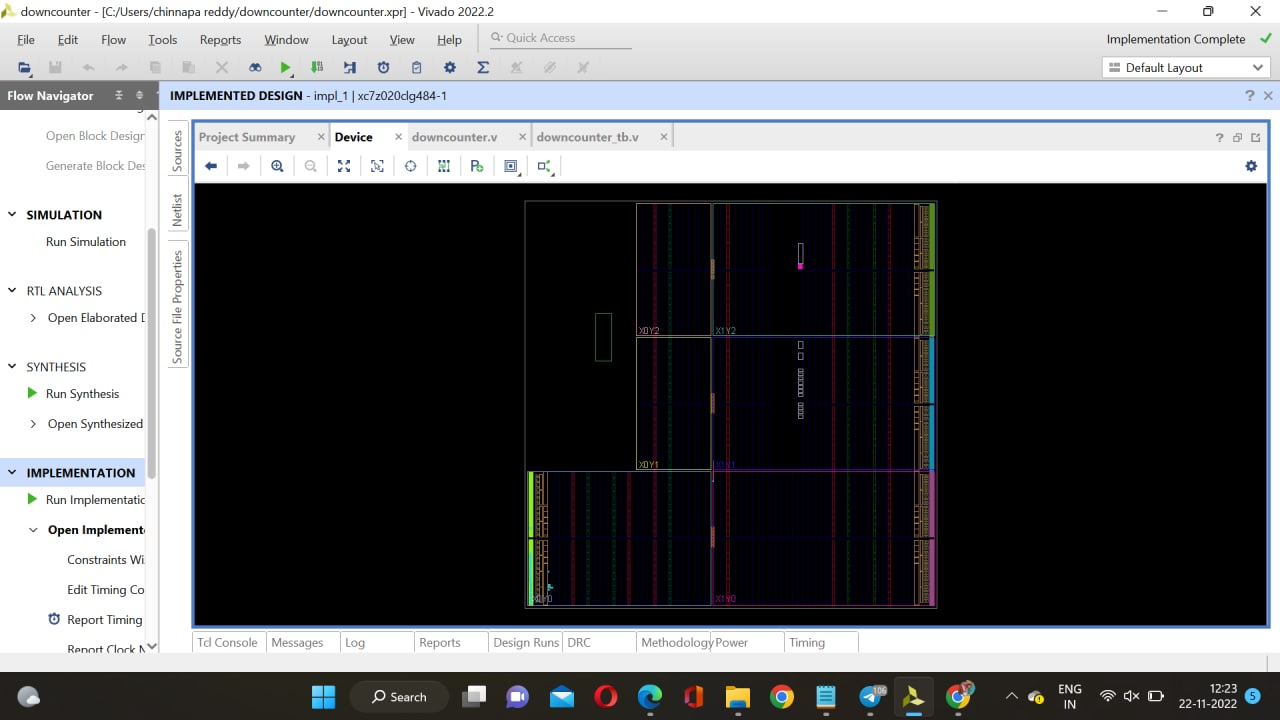
\includegraphics[width=1\columnwidth]{figs/2.jpg}
\section{Schematic diagram}
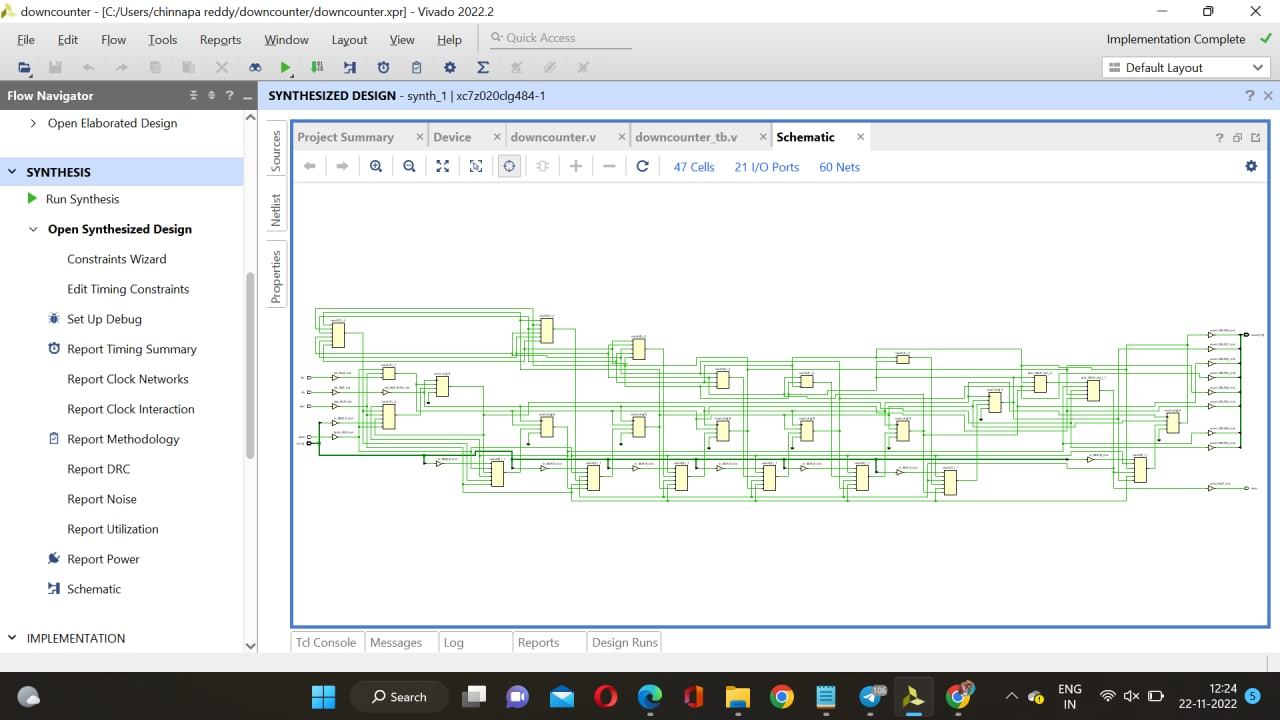
\includegraphics[width=1\columnwidth]{figs/3.jpg}
\end{document}

